\item \textbf{CodeBô: Design e avaliação de um puzzle game para o ensino de Estrutura de Dados}

O intuito do projeto CodeBô \cite{de2025codebo} foi desenvolver um jogo digital
isométrico de \emph{puzzles} que se baseia na mecânica do \emph{lightBot}, um
jogo mobile educacional conceituado, mecânica esta que consiste em selecionar
uma ordem de movimentos que o personagem deve executar para se mover até um
local específico.

O jogo CodeBô utiliza essas mecânicas para
ensinar conceitos como Pensamento Computacional, pilhas, filas e listas.
\cite{de2025codebo}

\begin{figure}[H]
	\centering
	\caption{Captura de tela do jogo CodeBô}
	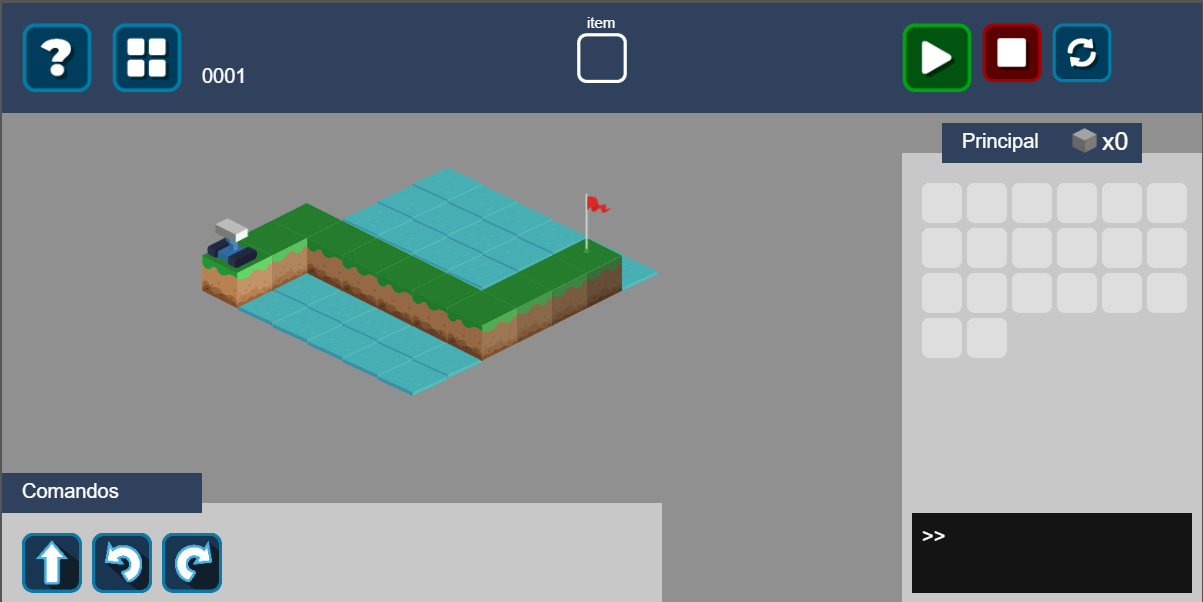
\includegraphics[width=0.8\textwidth]{images/codebo.png}
	\legend{Fonte: \cite{de2025codebo}}
	\label{fig:codebo}
\end{figure}


